\documentclass{ieeeaccess}
\usepackage{cite}
\usepackage{amsmath,amssymb,amsfonts}
\usepackage{algorithmic}
\usepackage{graphicx}
\usepackage{textcomp}
\def\BibTeX{{\rm B\kern-.05em{\sc i\kern-.025em b}\kern-.08em
    T\kern-.1667em\lower.7ex\hbox{E}\kern-.125emX}}
\begin{document}
\history{Date of publication xxxx 00, 0000, date of current version xxxx 00, 0000.}
\doi{10.1109/ACCESS.2017.DOI}

\title{Belief-Rule-Base Inference Method Based on Gradient Descent with Momentum}
\author{\uppercase{First A. Author}\authorrefmark{1}, \IEEEmembership{Fellow, IEEE},
    \uppercase{Second B. Author\authorrefmark{2}, and Third C. Author,
        Jr}.\authorrefmark{3},
    \IEEEmembership{Member, IEEE}}
\address[1]{National Institute of Standards and
    Technology, Boulder, CO 80305 USA (e-mail: author@boulder.nist.gov)}
\address[2]{Department of Physics, Colorado State University, Fort Collins,
    CO 80523 USA (e-mail: author@lamar.colostate.edu)}
\address[3]{Electrical Engineering Department, University of Colorado, Boulder, CO
    80309 USA}
\tfootnote{This paragraph of the first footnote will contain support
    information, including sponsor and financial support acknowledgment. For
    example, ``This work was supported in part by the U.S. Department of
    Commerce under Grant BS123456.''}

\markboth
{Author \headeretal: Preparation of Papers for IEEE TRANSACTIONS and JOURNALS}
{Author \headeretal: Preparation of Papers for IEEE TRANSACTIONS and JOURNALS}

\corresp{Corresponding author: First A. Author (e-mail: author@ boulder.nist.gov).}

\begin{abstract}

    The belief-rule-base (BRB) inference methodology using evidential reasonging (ER) approach is widely used in different fields,
    such as  fault diagnosis, system identification and decision analysis.
    Since the calculation of the individual matching degree in the inference process needs to set the reference value of the antecedent attribute,
    it is likely to cause the rule zero activation problem, and the intelligent algorithm for parameter training is not as efficient and accurate as the gradient method,
    but the partial derivative of inference system is difficult to construct.
    This paper propose a new belief rule structure and its gradient training method,
    aiming to solve zero activation problem during the inference process and improve inference accuray.
    Use Gaussian function to calculate the similarity of each attribute of the new rule structure instead of the original method.
    The characteristics of the Gaussian function avoid avoid the zero activation problem caused by the attribute reference value setting in the original method.
    On the basis of the new method, the corresponding distance-sensitive parameter is set for each attribute, and the weight parameter of each rule is discarded.
    It simplifies the calculation of rule activation weights in the inference process and enables the partial derivatives of the parameters of the inference system to be easily constructed.
    In the parameter optimization, the momentum optimization gradient stochastic descent method is used to train the new BRB system, which improves the training speed and accuracy compared with the conventional method.
    Experiments on non-linear function fitting, oil pipeline leak detection and several public classification datasets are conducted to validate
    the new BRB system trained by stochastic gradient descent with momentum (SGDM-BRB) has better performence compared with others conventional methods.
    The experimental results show that the SGDM-BRB has higher accuray and faster training speed than conventional method.

\end{abstract}

\begin{keywords}
    belief rule base, structure optimization, stochastic gradient descent, momentum optimization.
\end{keywords}

\titlepgskip=-15pt

\maketitle

\section{Introduction}
\label{sec:introduction}

It is well known that rule-based intelligent systems are one of the most common frameworks for expressing various types of knowledge.
The rule-based system has certain expression and processing capabilities through the use of existing human knowledge,
and at the same time has the flexibility to deal with ambiguity, incompleteness, uncertainty and to combine different types of input data formats.
In various rule-based systems for solving complex problems, belief rule-based inference methodology using evidential reasonging approach (ER) proposed by Yang \textit{et al}.\cite{a1}
baesd on conventional IF-THEN rules\cite{a2}, Dempster-Shafer theory of evidence\cite{a3,a4}, decision theory\cite{a5}
and fuzzy set theory\cite{a6} shows its powerful function of representing and processing uncertain information.
By introducing a belief distribution structure in the rules,
this methodology can effectively handle incomplete and uncertain information involved in the datasets and
widely used in various problem in different fields such as
oil pipeline leak detection\cite{a7}, military capability estimation\cite{a8}, consumer behavior prediction\cite{a9} and so on.

In the inference process of the belief rule base (BRB) system, the attribute weight, rule weight, belief distribution and other parameters
directly affect the final accuray. Yang \textit{et al}.\cite{a10} proposed optimization models for training BRB system using fmincon solver in
Matlab, Chang \textit{et al}.\cite{a11,a12} proposed an algorithm for training parameters in BRB system based on gradient and dichotomy methods,
Wu \textit{et al}.\cite{a13} used the accelerating of gradient algorithm to improve the convergence accuray and convergence speed. There are also
a series of intelligent algorithms such as the particle swarm algorithm proposed by Su \textit{et al}.\cite{a14} and the differential evolution
algorithm proposed by Wang \textit{et al}.\cite{a15} have excellent training performance on the BRB system.
Liu \textit{et al}.\cite{a16} introduces the belief distribution structure into the antecedent attributes and
uses training data to build an extended belief rule base (EBRB) system,
which simplifies the construction of the rule base and improves the inference speed.

At present, the parameter optimization of the BRB system is mostly based on various intelligent algorithms.
However, the process of those intelligent algorithms is complicated and there are many intermediate training parameters.
When the conventional gradient method trains the parameters of the BRB system, the partial derivative of each parameter is difficult to construct,
and the limit method is needed to solve the approximate value of the partial derivative\cite{a13}.
The step size is limited by the corresponding parameter constraints and a search is required to find the best effective step size\cite{a11,a12,a13}.
The EBRB system does not introduce a parameter training process, which makes the system have higher requirements for the representativeness of the training data used to construct the rule base.
For a large number of rules, it is necessary to perform rule reduction or use the data structure to optimize the storage and activation process of the rules.
Due to the conventional BRB system rule attribute reference level setting, its potential zero activation problem may cause the inference system to malfunction.

In response to the above problems, a series of optimization modifications are proposed for the system structure and reasoning process, including:

\quad 1) A new antecedent structure that does not need to set the attribute reference level is proposed, and a Gaussian function-based
rule weight activation method is proposed for the new rule antecedent structure. It effectively avoid the zero activation problem and has the feature of
generating rules from the training data like EBRB.

\quad 2) Setting the global weight parameters for antecedent attributes is cancelled,
and each rule is set with its own antecedent attribute weight parameters,
so that each rule has a better activation granularity.
On this basis, the setting of rule weight parameters and the related normalization process are cancelled,
which simplifies the evidential reasoning process.

\quad 3) Aa normalized exponential function is proposed to preprocess the restricted parameters to
avoid the problem of parameter failure during the training process.

The remainder of this paper is organized as follows: Section II introduces the conventional BRB system and our further improvements for common problems in the system.
Section III gives the preprocessing method of the training model and prove that the gradient descent method can be effectively applied to the newly proposed BRB system.
Section IV compares the performance of different gradient descent parameters on training speed and inference accuracy. Experiments on a series of public datasets prove that
the newly proposed BRB model and its training method have a better performance than other conventional methods. Section V concludes this paper.


\section{BRB system with new attribute structure and rule activation weight calculation method}
The BRB system proposed by Yang \textit{et al}.\cite{a1} mainly refers to the rule activation and evidence reasoning method on the belief rule base.
This section will briefly introduce the related concepts of the BRB system and propose the solutions for the common defects of the conventional BRB system.
\subsection{representation of belief rule base}
On the basis of the conventional production rules, Yang \textit{et al}.\cite{a1} proposed the expression form of the belief rules by introducing the belief distribution structure,
the rule antecedent attribute parameter and the rule weight parameter. The specific expression is as follows:
\begin{equation}
    \begin{split}
        &R_k:if\{X_1isA_1^k \wedge \cdots \wedge X_{T_k}isA_{T_k}^k\} \\
        &then\{(D_1,\beta_1^k),\cdots,(D_N,\beta_N^k)\},\sum_{i=1}^N\beta_i^k\leq1
    \end{split}
\end{equation}

The equal sign is obtained when the rule information is complete. Each rule has its rule weight $\theta_k$ and each antecedent attribute has its weight $\delta_{1},\delta_{2},\cdots,\delta_{T_k}$.
$A_i^k$ represents the reference value selected by the rule on the $i$-th attribute and $\beta_i^k$ represents the belief degree of the rule in the $i$-th consequent attribute.
On this basis, the extended belief rule base system introduces a belief distribution structure to the antecedent attributes, and its rule form is expressed as follows:
\begin{equation}
    \begin{split}
        &R_k:if\{[(A_{11}^k,\alpha_{11}^k),\cdots,(A_{1J_1}^k,\alpha_{1J_1}^k)] \wedge \\
        &\cdots \wedge [(A_{T_k1}^k,\alpha_{T_k1}^k), \cdots,(A_{T_kJ_{T_k}}^k,\alpha_{T_kJ_{T_k}}^k)]\}\\
        &then\{(D_1,\beta_1^k),\cdots,(D_N,\beta_N^k)\},\sum_{i=1}^N\beta_i^k\leq1
    \end{split}
\end{equation}
The extended belief rule base converts the original training data into antecedent attributes with a belief distribution form.
For the input data $X^k=(x_1^k,\cdots,x_T^k)$, convert the $i$-th attribute parameter to construct the $i$-th antecedent attribute of the corresponding rule in the form of belief distribution:
\begin{equation}
    \begin{split}
        &\alpha_{ij}^k=\frac{\gamma_{i(j+1)-x_i^k}}{\gamma_{i(j+1)-\gamma_{ij}}},\gamma_{ij}\leq x_i^k\leq \gamma_{i(j+1)}\\
        &\alpha_{i(j+1)}^k=1-\alpha_{ij}^k,\gamma_{ij}\leq x_i^k\leq \gamma_{i(j+1)} \\
        &\alpha_{it}^k=0,t=1,\cdots,(j-1),(j+2),\cdots,J_i
    \end{split}
\end{equation}
Using the same conversion method, the values of original data on other attributes can be converted into the corresponding belief distribution form.
It is also possible to obtain the belief distribution form of the rule consequent attribute according to this method.

\subsection{evidence reasoning approach based on belief rule base}
The calculation and synthesis of activation weights for each rule in the rule base is the core part of the inference system of the belief rule base.
The whole process mainly includes two steps: calculate the activation weight, and synthesize the rules activation weight to get the result.
The calculation of the activation weight of each rule in the belief rule base can be regarded as calculating the belief distribution similarity on each attribute and combining the results.
Euclidean distance is used to calculate the individual matching degree of the $i$-th attribute. After converting the input data to have the same belief distribution form as the corresponding attribute,
the individual matching degree of the attribute is calculated as:
\begin{equation}
    S_i^k=1-d_i^k=1-\sqrt{\frac{\sum_{j=1}^{J_i}(\alpha_{i,j}-\alpha_{i,j}^k)^2}{2}}
\end{equation}

After the individual matching degree of each attribute is calculated, the individual matching degrees of all attributes are aggregated. The aggregation function in the form of conjunctive rules is:
\begin{equation}
    \alpha_k=\prod_{i=1}^{T_k}(S_i^k)^{\overline{\delta_i}},\overline{\delta_i}=\frac{\delta_i}{\max_{j=1,\cdots,T_k}\delta_j}
\end{equation}
The activation weight of this rule is calculated by the following formula:
\begin{equation}
    w_k=\frac{\theta_k\alpha_k}{\sum_{l=1}^L\theta_l\alpha_l}
\end{equation}

Rule weight normalization operation makes all weights satisfy $0\leq w_k\leq 1,\sum w_k=1$.

After the rule weight calculation is completed, all the rules are synthesized and the inference result is obtained.
First, the belief distribution of the rule is transformed into the corresponding probability quality information:
\begin{align}
     & m_{j,k}=w_k\beta_j^k,j=1,\cdots,N                          \\
     & m_{D,k}=1-\sum_{j=1}^Nm_{j,k}=1-w_k\sum_{j=1}^{N}\beta_j^k \\
     & \overline{m}_{D,k}=1-w_k                                   \\
     & \widetilde{m}_{D,k}=w_k(1-\sum_{j=1}^N\beta_j^k)
\end{align}

$m_{j,k}$ represents the credibility of the $k$ rule on the $j$ consequent attribute,
where $\overline{m}_{D,k}$ represents the credibility that the $k$-th rule is not assigned to any consequent attribute,
and $\widetilde{m}_{D,k}$  represents the credibility of the missing reference attribute of the $k$-th rule.
The total uncertainty credibility is given by $m_{D,k}=\overline{m}_{D,k}+\widetilde{m}_{D,k}$.
Synthesize the credibility information of all rules and obtain the final belief result of each consequent attribute:
\begin{align}
     & m_j=k[\prod_{i=1}^L(m_{j,i}+m_{D,i})-\prod_{i=1}^Lm_{D,i}],j=1,\cdots,N       \\
     & \overline{m}_D=n[\prod_{i=1}^L\overline{m}_{D,i}]                             \\
     & \widetilde{m}_D=k[\prod_{i=1}^Lm_{D,i}-\prod_{i=1}^L\overline{m}_{H,i}]       \\
     & k=[\sum_{j=1}^N\prod_{i=1}^L(m_{j,i}+m_{D,i})-(N-1)\prod_{i=1}^Lm_{D,i}]^{-1} \\
     & \beta_j=\frac{m_j}{1-\overline{m}_D},j=1,\cdots,N                             \\
     & \beta_D=\frac{\widetilde{m}_D}{1-\overline{m}_D}
\end{align}

\subsection{new attribute structure and rule activation weight calculation method}
The reference value of antecedent attribute information needs to be set before generating rules.
If the input is not in the neighborhood of the reference value of the antecedent attribute of a rule, the rule cannot be activated.
If all the rules in rule base are not activated, the inference system will fail.
A simplified belief rules structure and corresponding activation weight calculation method is proposed to solve the above problems.
Its structure is as follows:
\begin{equation}
    \begin{split}
        &R_k:if(x_1^k , \cdots , x_{T_k}^k)\\
        &then\{(D_1,\beta_1^k),\cdots,(D_N,\beta_N^k)\},\sum_{i=1}^N\beta_i^k\leq1
    \end{split}
\end{equation}

The simplified belief rule structure can directly use the training data to generate the rule antecedent attribute without manually setting the reference values of the antecedent attributes.

The conventional activation weight calculation method is no longer suitable for the simplified form of belief rules.
The use of Gaussian function to calculate individual matching degree for activation weight calculation is proposed to perform weight activation.
The degree of individual matching of input $X(x_1,\cdots,x_{T_k})$ and rule $R_k:if(x_1^k , \cdots , x_{T_k}^k)then\{(D_1,\beta_1^k),\cdots,(D_N,\beta_N^k)\}$ on $i$-th attribute is calculated using the Gaussian function as:
\begin{equation}
    S_i^k=e^{-[a_i^k\times(x_i-x_i^k)]^2}
\end{equation}
The parameter $a_i^k$ represents the sensitivity of the $i$-th attribute to the distance at the position $x_i^k$. When the distance between the rule antecedent attribute and the input data remains unchanged,
the value of parameter $a$ inversely proportional to the matching degree.
The activation weight of a single rule under conjunctive conditions is calculated by the following formula:
\begin{equation}
    w_k=\prod_{i=1}^{T_k}S_i^k=e^{-\sum_{i=1}^{T_k}[a_i^k(x_i-x_i^k)]^2}
\end{equation}


\Figure[!t](topskip=0pt, botskip=0pt, midskip=0pt)[width=3.3 in]{fig_brb.eps}
{Activation weight calculated by conventional methods\label{fig1}}
\Figure[!t](topskip=0pt, botskip=0pt, midskip=0pt)[width=3.3 in]{fig_exp.eps}
{Activation weight calculated by Gaussian function methods with distance-sensitive parameter $a$ set to $1.0$\label{fig2}}
\Figure[!t](topskip=0pt, botskip=0pt, midskip=0pt)[width=3.3 in]{fig_exp_half.eps}
{Activation weight calculated by Gaussian function methods with distance-sensitive parameter $a$ set to $0.5$\label{fig3}}
Assuming a rule with two attributes x and y located at the $(0,0)$, the conventional method and Gaussian function method are used to calculate the activation weights.
Set the reference reference values on the x-attributes and y-attributes to be $[-4,-3,-2,-1,0,1,2,3,4]$.
Ignore the rule weight setting of the two methods.
The activation weight distributions shown in Figure \ref{fig1},
Figure \ref{fig2} with distance-sensitive parameter $a$ set to $1.0$ and
Figure \ref{fig3} with distance-sensitive parameter $a$ set to $0.5$ can be obtained.

Figure \ref{fig1} shows that if the input on a certain attribute is not in the neighborhood of the rule attribute,
the activation weight of this rule fluctuates around zero and gets zero when the attribute gets a reference value.
If the activation weight of all rules is zero, the inference cannot be performed.
However, the weight in Figure \ref{fig2} and Figure \ref{fig3} smoothly drops close to zero according to the distance from the rule and will not take a value of zero.
Moreover, different distance-sensitive parameters enable the rule to adapt to the calculation of activation weights at different scales.
It eliminates the impact of rule zero activation on system inference performance,
improves the fitting performance of the inference system by adding the distance-sensitive parameters.

Another benefit brought by the new rule structure and activation weight calculation method is that
there is no need to adjust the activation weight of the rule by the attribute weight and rule weight.
By adjusting the distance-sensitive parameters on each attribute of each rule, a good activation effect and activation granularity can be obtained.
Due to the characteristics of the Gaussian function, the activation weight of each rule belongs to $(0, 1]$ without normalization operations.
It greatly simplifies the redundant weight adjustment and calculation in the inference process.


\section{Momentum optimized Gradient descent training parameter}
When the conventional gradient method is applied to the parameter training process of the inference system of the belief rule base,
it is difficult to construct the partial derivative formula of the rule attribute and the training step is restricted by the parameter constraints.
Compared with the conventional BRB system, the newly proposed rule structure with its activation weight calculation methid make it easier to construct the partial derivative of each part of the parameter.

There are four subsections in this section, including:

\quad 1) Calculating the partial derivatives of the parameters of the new BRB system.

\quad 2) Proving the differentiability of new BRB system.

\quad 3) Proposing exponential normalization function for preprocessing to avoid specific constraints during parameter training.

\quad 4) Proposing a parameter training method using stochastic gradient descent with momentum optimization.


\subsection{Partial derivative of the parameters of the brb system}
The inference process of the improved BRB system is shown in Figure \ref{infsys}.
According to the inference process and compound function chain derivation rules, the partial derivatives of the output to the different parameters of the system can be obtained.
\Figure[!t](topskip=0pt, botskip=0pt, midskip=0pt)[width=3.3 in]{process1.png}
{Inference system operation process\label{infsys}}

Since the model construction and experiment in this paper are carried out with complete data and
the rule consequent attribute does not include uncertain information, for any $k$-th rule:
\begin{equation}
    \sum_{i=1}^N\beta_{ik}=1(k=1,\cdots,L)
\end{equation}
\begin{equation}
    m_{D,k}=\overline{m}_{D,k},\widetilde{m}_{D,k}=0
\end{equation}
In the case of completeness, the $j$-th consequent attribute is expressed as:
\begin{equation}
    \beta_j=\frac{\prod_{i=1}^L(m_{j,i}+m_{D,i})-\prod_{i=1}^Lm_{D,i}}{\sum_{t=1}^N\prod_{i=1}^L(m_{t,i}+m_{D,i})-N\times\prod_{i=1}^Lm_{D,i}}
\end{equation}
Then the result of the $j$-th consequent attribute before normalization is expressed as:
\begin{equation}
    \overline{\beta}_j = \prod_{i=1}^L(m_{j,i}+m_{D,i})-\prod_{i=1}^Lm_{D,i},\beta_j=\frac{\overline{\beta}_j}{\sum_{k=1}^N\overline{\beta}_k}
\end{equation}
Substitute $m_{j,i}=w_i\beta_{j,i}$ and $m_{D,i}=1-w_i$ into the $j$-th consequent attribute before normalization expression:
\begin{equation}
    \overline{\beta}_j = \prod_{i=1}^L(w_i\beta_j^i+1-w_i)-\prod_{i=1}^L{(1-w_i)}
\end{equation}
Obtain the partial derivative of the $i$-th consequent attribute $\beta_i$ to the $j$-th unnormalized consequent attribute $\overline{\beta}_j$:
\begin{equation}
    \frac{d\beta_i}{d\overline{\beta}_j}=
    \left\{
    \begin{aligned}
        \frac{\sum_{k\neq j}^N\overline{\beta}_k}{(\sum_{k=1}^N\overline{\beta}_k)^2},j=i \\
        -\frac{\beta_i}{(\sum_{k=1}^N\overline{\beta}_k)^2},j\neq i
    \end{aligned}
    \right.
\end{equation}
Similarly, the partial derivative of the $j$-th unnormalized consequent attribute $\overline{\beta}_j$ to the activation weight of the $k$-th rule and the $j$-th consequent attribute of $k$-th rule can be obtained as:
\begin{align}
     & \frac{d\overline{\beta}_j}{dw_k}=(\beta_j^k-1)\prod_{i=1,i\neq k}^L(w_i\beta_j^i+1-w_i)+\prod_{i=1,i\neq k}^L(1-w_i) \\
     & \frac{d\overline{\beta}_j}{d\beta_j^k}=w_k\prod_{i=1,i\neq k}^L(w_i\beta_j^i+1-w_i)
\end{align}
According to the activation weight expression of the $k$-th rule, the partial derivatives of the rule antecedent attribute parameter and the corresponding attribute distance-sensitive parameter can be obtained respectively:
\begin{align}
     & \frac{dw_k}{dx_l^k}=2(a_l^k)^2(x_l-x_l^k)e^{-\sum_{i=1}^{T_k}[a_i^k(x_i-x_i^k)]^2}  \\
     & \frac{dw_k}{da_l^k}=2a_l^kx_l^k(x_l-x_l^k)e^{-\sum_{i=1}^{T_k}[a_i^k(x_i-x_i^k)]^2}
\end{align}
Set the loss function expression of the final output to be $loss=Loss(\beta_1,\cdots,\beta_N)$.
According to the compound function chain derivation rule, the partial derivative of the final loss on each parameter can be obtained.
\begin{align}
     & \frac{dloss}{d\beta_j^k}=\sum_{i=1}^N\sum_{j=1}^N\frac{dloss}{d\beta_i}\frac{d\beta_i}{d\overline{\beta}_j}\frac{d\overline{\beta}_j}{d\beta_j^k}          \\
     & \frac{dloss}{dx_l^k}=\sum_{i=1}^N\sum_{j=1}^N\frac{dloss}{d\beta_i}\frac{d\beta_i}{d\overline{\beta}_j}\frac{d\overline{\beta}_j}{dw_k}\frac{dw_k}{dx_l^k} \\
     & \frac{dloss}{da_l^k}=\sum_{i=1}^N\sum_{j=1}^N\frac{dloss}{d\beta_i}\frac{d\beta_i}{d\overline{\beta}_j}\frac{d\overline{\beta}_j}{dw_k}\frac{dw_k}{da_l^k}
\end{align}

\subsection{Differentiable proof of BRB system}
The evidential reasoning process of the belief rule base system is a multivariate compound function process.
According to the differentiable condition of the multivariate compound function, each intermediate function must satisfy the differential condition,
and the partial derivative of each parameter must exist and be continuous.
Since any of the partial derivatives above are only obtained by elementary functions through four arithmetic operations and compound,
the partial derivatives of any parameter are continuous in its domain.
The existence and continuous partial derivative of any parameter can prove that the whole inference system is differentiable.

When the appropriate loss function is selected, the final output loss is differentiable to all the parameters of the model,
which provides conditions for using the gradient method to optimize the model parameters.
The gradient of the loss result on the parameters of each part of the model can be obtained.
The gradient of the loss function on all the rule antecedent attribute parameters is:
\begin{equation}
    \nabla_{x}loss=\left[\begin{matrix}
            \frac{dloss}{dx_1^1} & \cdots & \frac{dloss}{dx_{T_k}^1} \\
            \vdots               & \ddots & \vdots                   \\
            \frac{dloss}{dx_1^L} & \cdots & \frac{dloss}{dx_{T_k}^L}
        \end{matrix}\right]
\end{equation}
The gradient of the loss function on the distance-sensitive parameters of all rules is:
\begin{equation}
    \nabla_{a}loss=\left[\begin{matrix}
            \frac{dloss}{da_1^1} & \cdots & \frac{dloss}{da_{T_k}^1} \\
            \vdots               & \ddots & \vdots                   \\
            \frac{dloss}{da_1^L} & \cdots & \frac{dloss}{da_{T_k}^L}
        \end{matrix}\right]
\end{equation}
The gradient of the loss function on all rule consequent attribute parameters is:
\begin{equation}
    \nabla_{\beta}loss=\left[\begin{matrix}
            \frac{dloss}{d\beta_{1,1}} & \cdots & \frac{dloss}{d\beta_{N,1}} \\
            \vdots                     & \ddots & \vdots                     \\
            \frac{dloss}{d\beta_{1,L}} & \cdots & \frac{dloss}{d\beta_{N,L}} \\
        \end{matrix}\right]
\end{equation}

According to the belief distribution output by the inference system and the loss function of the result,
the gradient of each part of the parameters can be optimized by updating the parameters along the negative gradient direction.

\subsection{Exponential normalization function preprocessing}
In the training process, in order to satisfy the restriction that the sum of the consequent attributes of each rule is one and each consequent attribute is non-negative,
the exponential normalization function is used to preprocess the consequent attributes:
\begin{equation}
    \beta_j^k=\frac{e^{\overline{\beta_j^k}}}{\sum_{i=1}^Ne^{\overline{\beta_i^k}}}(\sum_{i=1}^N\beta_j^k=1,\beta_j^k>0)
\end{equation}
The derivative of the corresponding parameter can be obtained through the formula:
\begin{equation}
    \frac{d\beta_j^k}{d\overline{\beta_t^k}}=
    \left\{
    \begin{aligned}
        \beta_t^k\times(1-\beta_j^k),t=j \\
        -\beta_t^k\times\beta_j^k,t\neq j
    \end{aligned}
    \right.
\end{equation}
The partial derivative of the unpreprocessed consequent attribute can be expressed as:
\begin{equation}
    \frac{dloss}{d\overline{\beta_j^k}}=\sum_{i=1}^N\sum_{t=1}^N\frac{dloss}{d\beta_i}\frac{d\beta_i}{d\overline{\beta}_t}\frac{d\overline{\beta}_t}{d\beta_t^k}\frac{d\beta_t^k}{d\overline{\beta_j^k}}
\end{equation}
Also according to the elementary function chain derivation rule, the derivative of this parameter is continuous in its domain,
and the parameter is differentiable. Its gradient is expressed as:
\begin{equation}
    \nabla_{\overline{\beta}}loss=\left[\begin{matrix}
            \frac{dloss}{d\overline{\beta_1^1}} & \cdots & \frac{dloss}{d\overline{\beta_N^1}} \\
            \vdots                              & \ddots & \vdots                              \\
            \frac{dloss}{d\overline{\beta_1^L}} & \cdots & \frac{dloss}{d\overline{\beta_N^L}} \\
        \end{matrix}\right]
\end{equation}


\subsection{Stochastic gradient descent with momentum optimization}
The optimization process of using the gradient descent method to update the parameters of the inference model is given by the following equation:
\begin{equation}
    M_{new}(x,a,\beta)=M_{old}-\mu\nabla_{M_{old}}loss
\end{equation}

The gradient is given according to the loss function of the final output,
and the learning rate $\mu$ is the updated step length that needs to be set.
Chang and Zhang\cite{a11} and Wu \textit{et al}.\cite{a13} used dichotomy in the gradient training process to iteratively find the optimal step size in the constraint space and
added perturbation parameters when the gradient is zero to avoid the training process stagnation.
For the application of new rule structures, activation methods and preprocessing steps, the gradient training update step size is no longer limited.
The momentum-optimized stochastic gradient descent method is proposed for faster training.

The stochastic gradient descent method is an iterative optimization method when the objective function is differentiable.
It used a random subset of the training data to calculate the gradient value as the estimated value of the entire training data gradient,
which reduces the computational burden in high-dimensional optimization problems.

The output of the loss function in the conventional gradient descent method is determined by all samples,
and the model parameters are updated according to its gradient:
\begin{equation}
    loss=\frac{1}{n}\sum_i^nLoss(\beta_1^i,...,\beta_N^i)
\end{equation}
Randomly select a single sample as the estimated value of the average value of the loss function output on all samples to update the model parameters:
\begin{equation}
    loss=Loss(\beta_1^r,...,\beta_N^r)
\end{equation}
Since the update direction completely depends on the gradient of the current sample, the stochastic gradient descent method is not stable.
The momentum method improves the stability and speed by retaining a certain degree of historical gradient information and combining it with the current sample gradient.
It also enhances the ability to get rid of local optimal solutions.

The momentum method uses a weighted fusion method to synthesize the historical gradient information and the current sample gradient,
and use it as an update parameter for each round of training:
\begin{equation}
    v_t=\nu v_{t-1}+\mu\nabla_{loss}M,M=M-v_t
\end{equation}

The initial value of $v_0$ is set to zero and $\nu$ represent the ratio of retaining historical gradient information.
The same direction of the current gradient and the historical gradient will increase the speed of parameter training in this gradient direction.
The different directions of the current gradient and the historical gradient will inhibit the current gradient from causing parameter training oscillations.

\section{experimental results}
This section first compares the training performance of the gradient method under different momentum parameters through a nonlinear function fitting experiment,
and then compares the performance of the SGDM-BRB system under different parameter settings through the oil leak detection experiment.
Finally the SGDM-BRB system is compared with conventional machine learning algorithms on several public classification datasets and all experimental results are summarized.

\subsection{experimental enviroment}
The experiment runs on a Ubuntu 20.04 system equipped with Intel$^{\copyright}$ Core$^{\text{TM}}$ i5 8500@3.0GHz CPU, 16GB RAM and GeForce GTX 1060 Graphics.
Use TensorFlow 2 to build the evidential reasoning framework of the BRB system and use Scikit-learn machine learning library to collect and clean datasets.

\subsection{performance of gradient descent method with different momentum parameters}
Liu \textit{et al}.\cite{a16} proved that the belief rule base system can approximate any function.
In this section, a nonlinear multi-extreme function is introduced to compare the training performance of the stochastic gradient descent method under different momentum parameters.
The nonlinear multi-extreme function is as follows:
\begin{equation}
    f(x)=e^{-(x-2)^2}+0.5e^{-(x+2)^2},x\in[-5,5]
    \label{f_exp}
\end{equation}

\subsubsection{Basic Settings And Optimization}
In the domain defined by function \eqref{f_exp}, $1000$ sample data are uniformly selected as the fitting dataset and the mean square error is used as the loss function.
According to each extreme point on the function curve, the rule base consequent attribute evaluation level and corresponding utility value can be set:
$$\{D_1,D_2,D_3,D_4,D_5\}=\{-0.5,0,0.5,1,1.5\}$$
Select the five extreme points on the function curve to convert to the corresponding rule structure to build a belief rule base.
Set the default distance-sensitive parameter of each rule to $1.0$.
The initial rule information is shown in Table \ref{tab1}. Figure \ref{fig4} shows the untrained brb system output.
Set the number of training samples in each batch to be $128$ and the learning rate $\mu$ to be $0.001$ for $1000$ rounds of training.
Set the momentum optimization parameters $\nu$ to be 0.0 (non momentum optimization), $0.5$, $0.9$ and $0.99$ to compare their fitting performance.

\begin{table*}
    \caption{Initial rule information}
    \centering
    \normalsize
    \label{tab1}
    \begin{tabular}{cccccccc}
        \hline
        No. & Antecedent attribute $x$ & Distance-sensitive $a$ & \multicolumn{5}{c}{Consequent attributes $\overline{\beta}$}                         \\
        \hline
        $1$ & $-5$                     & $1$                    & (-1,                                                         & 1,  & -1, & -1, & -1) \\
        $2$ & $-2$                     & $1$                    & (-1,                                                         & -1, & 1,  & -1, & -1) \\
        $3$ & $0$                      & $1$                    & (-1,                                                         & 1,  & -1, & -1, & -1) \\
        $4$ & $2$                      & $1$                    & (-1,                                                         & -1, & -1, & 1,  & -1) \\
        $5$ & $5$                      & $1$                    & (-1,                                                         & 1,  & -1, & -1, & -1) \\
        \hline
    \end{tabular}
\end{table*}

\Figure[!t](topskip=-10pt, botskip=-10pt, midskip=0pt)[width=3.3 in]{initial_brb.png}
{Untrained BRB system output\label{fig4}}

\subsubsection{Results And Analysis}
\Figure[!t](topskip=-10pt, botskip=-10pt, midskip=0pt)[width=3.3 in]{mse.png}
{Mean square error loss under different momentum parameters\label{fig5}}
Figure \ref{fig5} shows the mean square error loss of each batch under different momentum parameters.
Through the decreasing curve of the mean square error loss function,
it can be found that smaller momentum optimization parameters can significantly improve the model performance.
The loss of the model with the momentum parameter set to $0.5$ has never been lower than 0.001 during the training process.
The loss of the model with the momentum parameter set to $0.9$ and $0.99$ dropped rapidly to $1\times10^{-4}$,
and reached the level of $1\times10^{-5}$ when the training is over.

Figure \ref{fig6} shows that higher momentum parameter values can obtain better fitting performance,
greatly reducing the distance between the fitted curve and the original curve.
\Figure[!t](topskip=-10pt, botskip=-10pt, midskip=0pt)[width=3.3 in]{fit.png}
{Fitting performance of different momentum parameter models\label{fig6}}

Table \ref{tab2} records the information of each rule in the model with the momentum parameter set to $0.99$ when the training is completed.
The distance-sensitive parameters have become smaller after training, that is, the activation area of each rule has increased.
The consequent attribute in their respective utility levels is significantly increased , while other levels have decreased.
The antecedent attribute information of each rule is only slightly adjusted after training.

\begin{table*}
    \caption{Trained rule information}
    \centering
    \normalsize
    \label{tab2}
    \begin{tabular}{cccccccc}
        \hline
        No. & Antecedent attribute $x$ & Distance-sensitive $a$ & \multicolumn{5}{c}{Consequent attributes $\overline{\beta}$}                                       \\
        \hline
        $1$ & $-4.55$                  & $0.207$                & (0.101,                                                      & 1.58,  & -1.83, & -1.73,  & -1.74)  \\
        $2$ & $-2.01$                  & $0.446$                & (-1.35,                                                      & -1.54, & 0.562, & -0.461, & -0.478) \\
        $3$ & $0.0805$                 & $0.509$                & (-0.154,                                                     & 1.48,  & -1.55, & -1.52,  & -1.61)  \\
        $4$ & $2.06$                   & $0.498$                & (-1.81,                                                      & -2.06, & -1.97, & 1.54,   & 0.597)  \\
        $5$ & $4.75$                   & $0.214$                & (0.123,                                                      & 1.55,  & -1.83, & -1.74,  & -1.78)  \\
        \hline
    \end{tabular}
\end{table*}

Table \ref{tab3} compares the performance of the SGDM-BRB with several conventional BRB system,
including the final mean square error results and training time of these models.
It is obvious that the gradient method after the momentum optimization has excellent performance in improving the inference accuracy of the BRB system,
but the training model without the effective momentum parameter optimization cannot reach the loss level of the conventional method.
And the running speed of gradient method is much lower than the conventional BRB system optimized by intelligent algorithm and other gradient descent algorithm.

\begin{table}
    \caption{Mean square error and training time using different optimization algorithms}
    \centering
    \label{tab3}
    \begin{tabular}{cccc}
        \hline
        Year       & Method             & Mean square error     & Running time \\
        \hline
        2007       & fmincon\cite{a10}  & $5.16\times10^{-5}$   & 496.17       \\
        2007       & Chen-BRB\cite{a13} & $6.3228\times10^{-5}$ & -            \\
        2015       & Wang-BRB\cite{a15} & $3.9284\times10^{-5}$ & 386.63       \\
        2018       & Li-BRB\cite{a36}   & $3.3322\times10^{-5}$ & 357          \\
        This study & SGD-BRB            & $5.90\times10^{-3}$   & 11.60        \\
        This study & SGDM-BRB(0.5)      & $3.50\times10^{-3}$   & 10.82        \\
        This study & SGDM-BRB(0.9)      & $4.01\times10^{-5}$   & 11.09        \\
        This study & SGDM-BRB(0.99)     & $7.40\times10^{-6}$   & 13.42        \\
        \hline
    \end{tabular}
\end{table}

\subsection{oil pipeline leak detection of BRB system with different settings}
In this section, oil pipeline leak detection are applied to validate the SGDM-BRB and reveal its practicability,
and compare the performance of models under different types of distance-sensitive parameters.

The oil pipeline leak detection dataset is a common benchmark used for testing BRB system and its improvements.
There are $2008$ sets of sample data collect every $10$ seconds. Each sample includes three continuous variables: flow difference, pressure difference and leak size.
The flow difference and pressure difference are used as independent variables, and the leak size is used as the dependent variable.
By comparing the mean square errors of these two parameter settings and other conventional BRB system optimization methods,
it is verified that the model with distance-sensitive parameters for each rule have better performance than the model with uniform distance-sensitive parameters for each attribute.

\subsubsection{Basic Settings And Optimization}
Randomly select $500$ samples as the training set.
The distance-sensitive of flow difference and pressure difference are set to be $1.0$ and $0.01$.
There are 5 reference levels for leak size, including zero (Z), very small (VS), medium (M), high (H) and very high (VH).
The reference values are:
\begin{equation}
    D_{LS}\in \{(Z,0),(VS,2),(M,4),(H,6),(Vh,8)\}
\end{equation}
Randomly select $16$ samples from the training set and convert them into the belief rule form and build the corresponding rule base.
For flow difference and pressure difference information, convert them into antecedent attribute.
For the leak size, set the consequent attribute to be the negative value of the distance from leak size to corresponding reference value.
The corresponding rule for a sample with flow difference $fd$, pressure difference $pd$ and leak size $ls$ is expressed as:
\begin{equation}
    \begin{split}
        &R:If(fd,pd)Then\{(\overline{\beta_{Z}},-|ls-0|),(\overline{\beta_{VS}},-|ls-2|),\\
        &(\overline{\beta_{M}},-|ls-4|),(\overline{\beta_{H}},-|ls-6|),(\overline{\beta_{Z}},-|ls-8|)\}
    \end{split}
\end{equation}
The initial belief rule base inference results for training set are shown in Figure \ref{oil_compare_before}.

\Figure[!t](topskip=0pt, botskip=0pt, midskip=0pt)[width=3.3 in]{oil_compare_before.eps}
{Comparison of the initial model output and the leak size of the training set\label{oil_compare_before}}

In the training process, the mean square error is used as the loss function, each batch uses $32$ samples, and a total of $1000$ rounds of training.
A model with distance-sensitive parameter for each rule has a total of 144(16$\times$(2+2+5)) parameters to be trained,
and a model with uniform distance-sensitive parameters for each attribute has a total of 114(16$\times$(2+5)+2) parameters to be trained.
The output of the model with distance-sensitive parameters for each rule after training is shown in Figure \ref{oil_compare_after}.
\Figure[!t](topskip=0pt, botskip=0pt, midskip=0pt)[width=3.3 in]{oil_compare_after.eps}
{Comparison of the trained model output and the leak size on all samples\label{oil_compare_after}}

\subsubsection{Results And Analysis}
All of $2008$ samples and estimated output are shown in Figure \ref{oil_compare}, it can be observed that the results of the two are roughly the same,
especially during the time when the leak occurred.
Note that there is a large leak estimation error around the $1000$th sample,
which may be caused by noisy data.
\Figure[!t](topskip=-10pt, botskip=-10pt, midskip=0pt)[width=7 in]{oil_compare.eps}
{Estimated output and samples\label{oil_compare}}
\Figure[!t](topskip=-10pt, botskip=-10pt, midskip=0pt)[width=7 in]{oil_ae.eps}
{Absolute error between estimated output and samples\label{oil_ae}}


To further verify the validity of SGDM-BRB, $20$ independent experiments on two different distance-sensitive parameters settings methods are conducted.
Tabel \ref{oil_tab} list the comparison of results of some existing works and two proposed methods,
where the mean square error and mean absolute error are obtained from $2008$ samples.

For the method of using uniform distance-sensitive parameters for each attribute, the mean absolute error and the mean square error are both ranks in the top four.
For the method of setting distance-sensitive parameters for each rule respectively, the mean absolute error and the mean square error are both ranks in the top two.
It only lags behind JOPS in the mean absolute error, and only lags behind Bi-level BRB model in the mean square error.

Since the new method simplifies the structure of using reference values to construct the belief distribution of the antecedent attributes,
it reduces a large number of parameters compared with the conventional BRB model.
If a uniform distance-sensitive parameter is used for each attribute,
the number of parameters can still be greatly reduced without significantly reducing the inference accuracy.
However, compared with other newer methods, our method still needs to train a certain number of rule parameters to improve the inference accuracy and cannot achieve the ultimate parameter reduction.

In summary, the comparison of experimental results show that the proposed method  achieves higher inference accuracy,
and a large number of parameters are reduced through simplification based on the traditional rule structure.

\begin{table*}
    \caption{Comparison wih present researches}
    \centering
    \label{oil_tab}
    \begin{tabular}{cccccc}
        \hline
        Year       & Method                                             & Size(training/test) & Parameters & Mean absolute error & Mean square error \\
        \hline
        2007       & Local training\cite{a30}                           & 500/2008            & 353        & 0.2223              & 0.4049            \\
        2011       & Adaptive learning\cite{a31}                        & 500/2008            & 353        & 0.2064              & 0.3990            \\
        2013       & Extended BRB\cite{a16}                             & -/2008              & 18902      & 0.2169              & -                 \\
        2016       & Dynamic rule adjustment\cite{a32}                  & 900/2008            & 43         & 0.2080              & 0.4450            \\
        2017       & Bi-level BRB\cite{a33}                             & 500/2008            & 40         & 0.1941              & 0.2917            \\
        2018       & JOPS\cite{a34}                                     & 900/2008            & 43         & 0.1738              & 0.3998            \\
        This study & SGDM-BRB(uniform distance-sensitive parameters)    & 500/2008            & 114        & 0.2024              & 0.3496            \\
        This study & SGDM-BRB(respective distance-sensitive parameters) & 500/2008            & 144        & 0.1998              & 0.3469            \\
        \hline
    \end{tabular}
\end{table*}


\subsection{Experiment on public classification datasets}
This section selects 7 UCI public classification datasets that are widely used to valid the inference performance of SGDM-BRB method.
Table \ref{tab4} shows the detailed information of these classification datasets.
Repeat independent 10-fold cross-validation experiments for 20 times to obtain the final results.
The results for comparison are measured by average accuracy.

The results obtained by SGDM-BRB method will be compared with the results obtained by
other machine learning methods and belief rule base inference system.
The machine methods for comparison include KNN, Naive Bayes (NB) and C4.5, support vector machine (SVM)
and their results are cited from previous papers\cite{a22,a27}.
The BRB systems used for comparison include SRA-EBRB\cite{a20}, MVP-EBRB\cite{a21} and BA-EBRB\cite{a22}.

\begin{table*}
    \caption{Accuracy of SGDM-BRB compare with conventional classification approaches}
    \centering
    \normalsize
    \label{tab5}
    \begin{tabular}{|c|c|c|c|c|c|c|c|c|}
        \hline
                     & KNN               & NB                & C4.5     & SVM               & SRA-EBRB & MVP-EBRB & BA-EBRB  & SGDM-BRB          \\
        \hline
        iris         & 96.67(\textbf{1}) & 96.00(4)          & 96.00(4) & 96.67(\textbf{1}) & 94.80(8) & 95.87(6) & 95.26(7) & 96.50(3)          \\
        wine         & 96.05(5)          &                   &          & 96.40(4)          & 96.85(3) &          & 97.02(2) & 97.44(\textbf{1}) \\
        diabetes     & 74.09(3)          & 76.30(\textbf{1}) & 73.82(4) & 65.10(8)          & 71.71(7) & 72.59(5) & 72.32(6) & 75.29(2)          \\
        ecoli        & 85.71(\textbf{1}) & 85.42(4)          & 84.23(5) & 75.60(7)          & 84.85(5) & 85.61(2) &          & 85.43(3)          \\
        glass        & 66.63(7)          & 48.60(8)          & 66.82(6) & 68.69(5)          & 73.08(2) & 72.06(4) & 72.32(3) & 74.75(\textbf{1}) \\
        seeds        & 92.38(3)          & 91.43(5)          & 91.90(6) & 90.48(8)          & 91.24(7) & 92.38(3) & 93.95(2) & 94.02(\textbf{1}) \\
        yeast        & 58.22(3)          & 57.61(4)          & 55.39(7) & 43.26(8)          & 56.85(6) & 57.49(5) & 58.63(2) & 59.49(\textbf{1}) \\
        \hline
        Average rank & 3.28(2)           & 4.33(5)           & 5.33(6)  & 6.44(8)           & 5.42(7)  & 4.16(4)  & 3.66(3)  & 1.71(\textbf{1})  \\
        \hline
    \end{tabular}
\end{table*}

\begin{table}
    \caption{Details of the classification datasets}
    \centering
    \normalsize
    \label{tab4}
    \begin{tabular}{cccc}
        \hline
        Dataset name & \#Instances & \#Features & \#Classes \\
        \hline
        iris         & 150         & 5          & 3         \\
        wine         & 178         & 14         & 3         \\
        diabetes     & 768         & 9          & 2         \\
        ecoli        & 336         & 8          & 8         \\
        glass        & 214         & 10         & 6         \\
        seeds        & 210         & 8          & 3         \\
        yeast        & 1484        & 9          & 10        \\
        \hline
    \end{tabular}
\end{table}



\subsubsection{Basic Settings And Optimization}
To enable a unified classification process,  standardized operation are performed on each dataset:
\begin{equation}
    x'=\frac{x-\overline{x}}{\delta}
\end{equation}
where $\overline{x}$ is the mean of $x$ and $\delta$ is the standard deviation of $x$.
After standardization, the data on each attribute can be approximated to the standard normal distribution,
and the distance-sensitive parameter on all attributes can be conveniently set to $1.0$.
Then choose cross entropy as the loss function to train the BRB system.
For a multi-classification task with $N$ categories, the loss function on each sample $y$ and the corresponding prediction result $\overline{y}$ is defined as follows:
\begin{equation}
    Loss(y,\overline{y})=-\sum_{i=1}^Ny_{i}\log\overline{y}_i
\end{equation}

For the experiment on each dataset, $32$ samples are randomly selected from training set as the initial rule
and convert the classification result into the corresponding belief result distribution according to the above conversion method.
The rule corresponding to the $k$-th training sample
\begin{equation}
    X_k:(x_1,...,x_{T_k}),Y_k:c,1\leq c\leq N
\end{equation}
is expressed as:
\begin{equation}
    \begin{split}
        &R_k:if(x'_1,\cdots,x'_{T_k})\\
        &then\{(\overline{\beta_1^k},-1),\cdots,(\overline{\beta_{c-1}^k},-1),(\overline{\beta_c^k},1),(\overline{\beta_{c+1}^k},-1),\\
        &\cdots,(\overline{\beta_N^k},-1)\}\\
        &with\, distance-sensitive\, parameter(a^k_1,\cdots,a^k_{T_k})
    \end{split}
\end{equation}
Assign each rule its own distance-sensitive parameters on all attributes to obtain a finer inference granularity by increasing the number of parameters.

In the process of parameter optimization using momentum optimization stochastic gradient descent method,
the learning rate is set to $0.001$ and the momentum optimization parameter is set to $0.99$.
There are $128$ training samples in each batch, and $2000$ rounds trainings are performed on each dataset.

\subsubsection{Results And Analysis}
Table \ref{tab5} lists the classification accuracy of SGDM-BRB method and other machine learning methods include several conventional improved BRB methods.
Although the SGDM-BRB method is not always the best method, its ranking never fell out of the top $3$, and it is also the method with the highest average ranking.
As shown in Table \ref{tab5}, our method achieves higher accuracy than any other methods on the four datasets of
wine, glass, seeds, and yeast.
For the other results shown in Table \ref{tab5},
SGDM-BRB method achieves
an accuracy of $96.50\%$ on tthe dataset iris
which is worse than the $96.67\%$ accuracies obtained from KNN and SVM,
an accuracy of $85.43\%$ on dataset ecoli
which is worse than the $85.71\%$ accuracy obtained from KNN and the $85.61\%$ accuracy obtained from MVP-BRB,
and an accuracy of $75.29\%$ on dataset pima is worse than the $76.30\%$ accuracy obtained from NB.

Thanks to the fixed number of rules to be trained, the number of parameters for each data set experiment only increases linearly with the number of antecedent attributes and the number of consequent attributes,
It effectively avoids the problem of parameter explosion that the conventional BRB method may encounter.

\section{conclusion}
This paper proposes a new rule structure and its activation method with the corresponding momentum optimization gradient training method.
The new rule structure uses original data to directly form rules, it the problem of parameter explosion caused by too many reference value settings.
The rule activation weight calculation method improved by using Gaussian function has effectively improved the inference accuracy by introducing distance-sensitive parameters,
the characteristic of Gaussian function avoids the rule zero activation problem and simplifies the process of normalizing rule activation weights.
The new structure and optimization method make it easier to construct the partial derivatives of the inference system,
providing conditions for high-performance gradient training methods.
The further conclusions of this paper are summarized as follow:

\quad 1) Using the method of combining attribute distance-sensitive parameters and Gaussian function instead of
the conventional belief distribution method to calculate the individual matching degree effectively avoids the defect that
the conventional method may cause the individual matching degree to be 0.
This makes the activation weight change more gentle and has good fitting performance.

\quad 2) The stochastic gradient method combined with larger momentum optimization parameters greatly improves the accuracy and convergence speed of the model.

Due to its good fitting performance, future research will focus on using integrated methods to further improve inference performance and reduce potential over-fitting risks.

\begin{thebibliography}{00}

    \bibitem{a1} J. B. Yang, J. Liu, J. Wang, ``Belief rule-base inference methodology
    using the evidential reasoning approach-rimer,''
    \emph{IEEE Transactions on Systems, Man, and Cybernetics - Part A: Systems and Humans},
    2006, 2(36):266-285.

    \bibitem{a2} R. Sun, ``Robust reasoning: integrating rule-based and similarity-based
    reasoning,'' \emph{Artificial Intelligence},
    1995, 2(75):241-295.

    \bibitem{a3}  A. P. Dempster, ``A generalization of bayesian inference,''
    \emph{Journal of the Royal Statistical Society: Series B (Methodological)},
    1968, 2(30): 205-232.

    \bibitem{a4} G. Shafer, A. F. M. Smith, ``A mathematical theory of evidence[J],''
    \emph{Biometrics},
    1976, 3(32):703.

    \bibitem{a5} K. Yoon, C. L. Hwang, ``Multiple attribute decision making,''
    \emph{Thousand Oaks, CA: Sage Publications},
    1995.

    \bibitem{a6} L. Zadeh, ``Fuzzy sets,''
    \emph{Information and Control},
    1965, 3(8):338-353.

    \bibitem{a7} Z. J. Zhou, C. H. HU, J. B. Yang, , ``Online updating belief rule based
    system for pipeline leak detection under expert intervention,''
    \emph{Expert Systems with Applications},
    2009, 4(36):7700-7709.

    \bibitem{a8} J. Jiang, X. Li, Z. J. Zhou, ``Weapon system capability assessment
    under uncertainty based on the evidential reasoning approach,''
    \emph{Expert Systems with Applications},
    2011.

    \bibitem{a9} Y. Yang, C. Fu, Y. W. Chen, ``A belief rule based expert system
    for predicting consumer preference in new product development,''
    \emph{Knowledge-Based Systems},
    2016(94):105-113.

    \bibitem{a10} J. B. Yang, J. Liu, D. L. Xu, ``Optimization models for training
    belief-rule-based systems,''
    \emph{IEEE Transactions on Systems, Man, and Cybernetics - Part A: Systems and Humans},
    2007, 4(37):569-585.

    \bibitem{a11} R. Chang, S. Zhang, ``An Algorithm for Training Param eters in Belief Rule-bases Based on
    Gradient Methods with Optimization Step Size,''
    \emph{Journal of North China Institute of Water Conservancy and Hydroelectric Power},
    2011, 1(32):154-157.

    \bibitem{a12} R. Chang Y, H. Wang, J. B. Yang, ``An algorithm for training parameters
    in belief rule-bases based on the gradient and dichotomy methods,''
    \emph{Systems Engineering},
    2007.

    \bibitem{a13} W. K. Wu, L. H. Yang, Y. G. FU, ``Parameter Training Approach for Belief Rule Base Using the Accelerating of Gradient
    Algorithm,''
    \emph{Journal of Frontiers of Computer Science and Technology},
    2014, 8(8):989-1001.

    \bibitem{a14} SU Q, L. H. Yang, Y. G. FU, ``Parameter training approach based on variable particle swarm optimization
    for belief rule base,''
    \emph{Journal of Computer Applications},
    2014, 34(8):2161-2165.

    \bibitem{a15} H. J. Wang, L. H. Yang, Y. G. FU , ``Differential Evolutionary Algorithm for Parameter Training of Belief Rule Base under Expert Intervention,''
    \emph{Computer Science},
    2015, 42(5):88-93.

    \bibitem{a16} J. Liu, L. Martinez, A. C. Calzada, ``A novel beliefrule base representation, generation and its inference methodology,''
    \emph{Knowledge-Based Systems},
    2013(53):129-141.

    \bibitem{a17} H. Robbins, S. Monro, ``A stochastic approximation method,''
    \emph{The Annals of Mathematical Statistics},
    1951, 3(22):400-407.

    \bibitem{a18} K. C. Kiwiel, ``Convergence and efficiency of subgradient methods for quasiconvex minimization,''
    \emph{Mathematical Programming},
    2001,1(90):1-25.

    \bibitem{a19} D. E. Rumelhart, G. E. Hinton, R. J. Williams, ``Learning representations
    by back-propagating errors,''
    \emph{Nature},
    1986, 6088(323):533-536.

    \bibitem{a35} Y. W. Chen, J. B. Yang, D. L. Xu, ``On the inference and approximation properties of belief rule based system,''
    \emph{Information Sciences}, 2013, 234(11):121-135.

    \bibitem{a36} M. Li, Y. G. Fu, W. L. Liu, Y. J. Wu, ``Parameter Training  Approach for Belief Rule Base Based on the Cuckoo Search Algorithm,''
    \emph{Journal of Chinese Computer Systems}, 2018, 39(6):1149-1155.

    \bibitem{a20} Y. Q. Lin, Y. G. FU, ``A rule activation method for extended belief rule base based on improved similarity measures,''
    \emph{Journal of University of Science and Technology of China},
    2018, 48(1):21-27.

    \bibitem{a21} Y. Q. Lin, Y. G. FU, SU Q, ``A rule activation method for extended belief rule base with vp-tree and mvp-tree,''
    \emph{Journal of Intelligent and Fuzzy Systems},
    2017, 33(6):3695-3705.

    \bibitem{a22} W. Fang, X. Gong, Liu G, ``A balance adjusting approach of extended
    belief-rule-based system for imbalanced classification problem,''
    \emph{IEEE Access},
    2020, 8(19419049):41201-41212.

    \bibitem{a23} C. E. Shannon, ``A mathematical theory of communication,''
    \emph{Bell System Technical Journal},
    1948, 4(27):623-656.

    \bibitem{a24} A. Calzada, J. Liu, H. Wang, ``A new dynamic rule activation
    method for extended belief rule-based systems,''
    \emph{IEEE Transactions on Knowledge and Data Engineering},
    2015, 4(27):880-894.

    \bibitem{a25} L. H. Yang, J. Liu, ``New activation weight calculation and parameter optimization
    for extended belief rule-based system based on sensitivity analysis,''
    \emph{Knowledge and Information Systems},
    2018, 60(2):837-878.

    \bibitem{a26} Y. Wang, ``Parameter learning for an intuitionistic fuzzy belief rulebased
    systems based on weight and reliability,''
    \emph{Journal of Advanced Computational Intelligence and Intelligent Informatics},
    2019, 23(2):219-228.

    \bibitem{a27} H. Zhu, M. Xiao, L. H. Yang, X. Tang, Y. Liang, J. Li, ``A minimum centre distance rule activation method for extended
    belief rule-based classification systems,''
    \emph{Applied Soft Computing},
    2020, 91:106214.

    \bibitem{a28} Q. Jia, J. Hu, W. Zhang, ``A novel fault detection model based on atanassov’s intervalvalued
    intuitionistic fuzzy sets, belief rule base and evidential reasoning,''
    \emph{IEEE Access}, 2020, 8:4551-4567.

    \bibitem{a30} D. L. Xu, J. Liu, J. B. Yang, G. P. Liu, J. Wang, L. Jenkinson, R. Jun, ``Inference and learning methodology of belief-rule-based expert system for pipeline leak detection,''
    \emph{Expert System with Applications}, 2007, 32:103–113.

    \bibitem{a31} Y. W. Chen, J. B. Yang, D. L. Xu, Z. J. Zhou , D. W. Tang, ``Inference analysis and adaptive training for belief rule based system,''
    \emph{Expert System with Applications}, 2011,38:12845–12860.

    \bibitem{a32} Y. Wang M, L. H. Yang, Y. G. Fu, L. L. Chang, K. S. Chin, ``Dynamic rule adjustment approach for optimizing belief rule-base expert system,''
    \emph{Knowledge-Based Systems}, 2016, 96:40–60.

    \bibitem{a33} L. L. Chang, Z. J. Zhou, T. J. Liao, Y. W. Chen, H. Yu, L. H. Yang, ``Belief rule base structure and parameter joint learning under disjunctive assumption for non- linear complex system modeling,''
    \emph{IEEE Transactions on Systems, Man, and Cybernetics, Part A}, 2017, 99:1–13.

    \bibitem{a34} L. H. Yang, Y. Wang M, J. Liu, L. Mart´ınez, ``A joint optimization method on parameter and structure for belief-rulebased systems,''
    \emph{Knowledge-Based Systems}, 2018, 142:220–240.

    \bibitem{a29} G. Holmes, A. Donkin, I. H. Witten, ``WEKA: A machine learning workbench,
    in: Conference on Intelligent Information Systems,'' 2002.

\end{thebibliography}

\begin{IEEEbiography}[{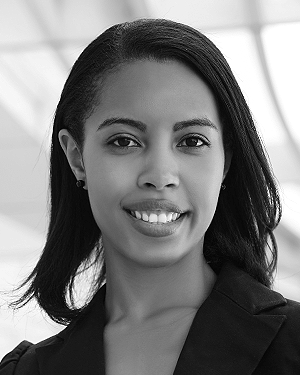
\includegraphics[width=1in,height=1.25in,clip,keepaspectratio]{a1.png}}]{First A. Author} (M'76--SM'81--F'87) and all authors may include
    biographies. Biographies are often not included in conference-related
    papers. This author became a Member (M) of IEEE in 1976, a Senior
    Member (SM) in 1981, and a Fellow (F) in 1987. The first paragraph may
    contain a place and/or date of birth (list place, then date). Next,
    the author's educational background is listed. The degrees should be
    listed with type of degree in what field, which institution, city,
    state, and country, and year the degree was earned. The author's major
    field of study should be lower-cased.

    The second paragraph uses the pronoun of the person (he or she) and not the
    author's last name. It lists military and work experience, including summer
    and fellowship jobs. Job titles are capitalized. The current job must have a
    location; previous positions may be listed
    without one. Information concerning previous publications may be included.
    Try not to list more than three books or published articles. The format for
    listing publishers of a book within the biography is: title of book
    (publisher name, year) similar to a reference. Current and previous research
    interests end the paragraph. The third paragraph begins with the author's
    title and last name (e.g., Dr.\ Smith, Prof.\ Jones, Mr.\ Kajor, Ms.\ Hunter).
    List any memberships in professional societies other than the IEEE. Finally,
    list any awards and work for IEEE committees and publications. If a
    photograph is provided, it should be of good quality, and
    professional-looking. Following are two examples of an author's biography.
\end{IEEEbiography}

\begin{IEEEbiography}[{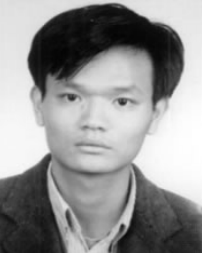
\includegraphics[width=1in,height=1.25in,clip,keepaspectratio]{a2.png}}]{Second B. Author} was born in Greenwich Village, New York, NY, USA in
    1977. He received the B.S. and M.S. degrees in aerospace engineering from
    the University of Virginia, Charlottesville, in 2001 and the Ph.D. degree in
    mechanical engineering from Drexel University, Philadelphia, PA, in 2008.

    From 2001 to 2004, he was a Research Assistant with the Princeton Plasma
    Physics Laboratory. Since 2009, he has been an Assistant Professor with the
    Mechanical Engineering Department, Texas A{\&}M University, College Station.
    He is the author of three books, more than 150 articles, and more than 70
    inventions. His research interests include high-pressure and high-density
    nonthermal plasma discharge processes and applications, microscale plasma
    discharges, discharges in liquids, spectroscopic diagnostics, plasma
    propulsion, and innovation plasma applications. He is an Associate Editor of
    the journal \emph{Earth, Moon, Planets}, and holds two patents.

    Dr. Author was a recipient of the International Association of Geomagnetism
    and Aeronomy Young Scientist Award for Excellence in 2008, and the IEEE
    Electromagnetic Compatibility Society Best Symposium Paper Award in 2011.
\end{IEEEbiography}

\begin{IEEEbiography}[{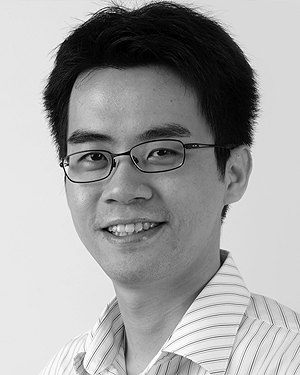
\includegraphics[width=1in,height=1.25in,clip,keepaspectratio]{a3.png}}]{Third C. Author, Jr.} (M'87) received the B.S. degree in mechanical
    engineering from National Chung Cheng University, Chiayi, Taiwan, in 2004
    and the M.S. degree in mechanical engineering from National Tsing Hua
    University, Hsinchu, Taiwan, in 2006. He is currently pursuing the Ph.D.
    degree in mechanical engineering at Texas A{\&}M University, College
    Station, TX, USA.

    From 2008 to 2009, he was a Research Assistant with the Institute of
    Physics, Academia Sinica, Tapei, Taiwan. His research interest includes the
    development of surface processing and biological/medical treatment
    techniques using nonthermal atmospheric pressure plasmas, fundamental study
    of plasma sources, and fabrication of micro- or nanostructured surfaces.

    Mr. Author's awards and honors include the Frew Fellowship (Australian
    Academy of Science), the I. I. Rabi Prize (APS), the European Frequency and
    Time Forum Award, the Carl Zeiss Research Award, the William F. Meggers
    Award and the Adolph Lomb Medal (OSA).
\end{IEEEbiography}

\EOD

\end{document}
